\documentclass{article}%
\usepackage[T1]{fontenc}%
\usepackage[utf8]{inputenc}%
\usepackage{lmodern}%
\usepackage{textcomp}%
\usepackage{lastpage}%
\usepackage[head=40pt,margin=0.5in,bottom=0.6in]{geometry}%
\usepackage{graphicx}%
%
\title{\textbf{Basura pone en riesgo la salud de los vecinos en Maracaibo}}%
\author{El Nacional Web}%
\date{06/10/2018}%
%
\begin{document}%
\normalsize%
\maketitle%
\textbf{URL: }%
http://www.el{-}nacional.com/noticias/sociedad/basura{-}pone{-}riesgo{-}salud{-}los{-}vecinos{-}maracaibo\_254633\newline%
%
\textbf{Periodico: }%
EN, %
ID: %
254633, %
Seccion: %
Sociedad\newline%
%
\textbf{Palabras Claves: }%
Aseo urbano, Salud, Zulia, Denuncia\newline%
%
\textbf{Derecho: }%
3.2%
, Otros Derechos: %
NO\_TIENE%
, Sub Derechos: %
3.2.1%
\newline%
%
\textbf{EP: }%
NO\newline%
\newline%
%
\textbf{\textit{Los habitantes denuncian que varias zonas llevan más de 18 días sin recibir el servicio de aseo}}%
\newline%
\newline%
%
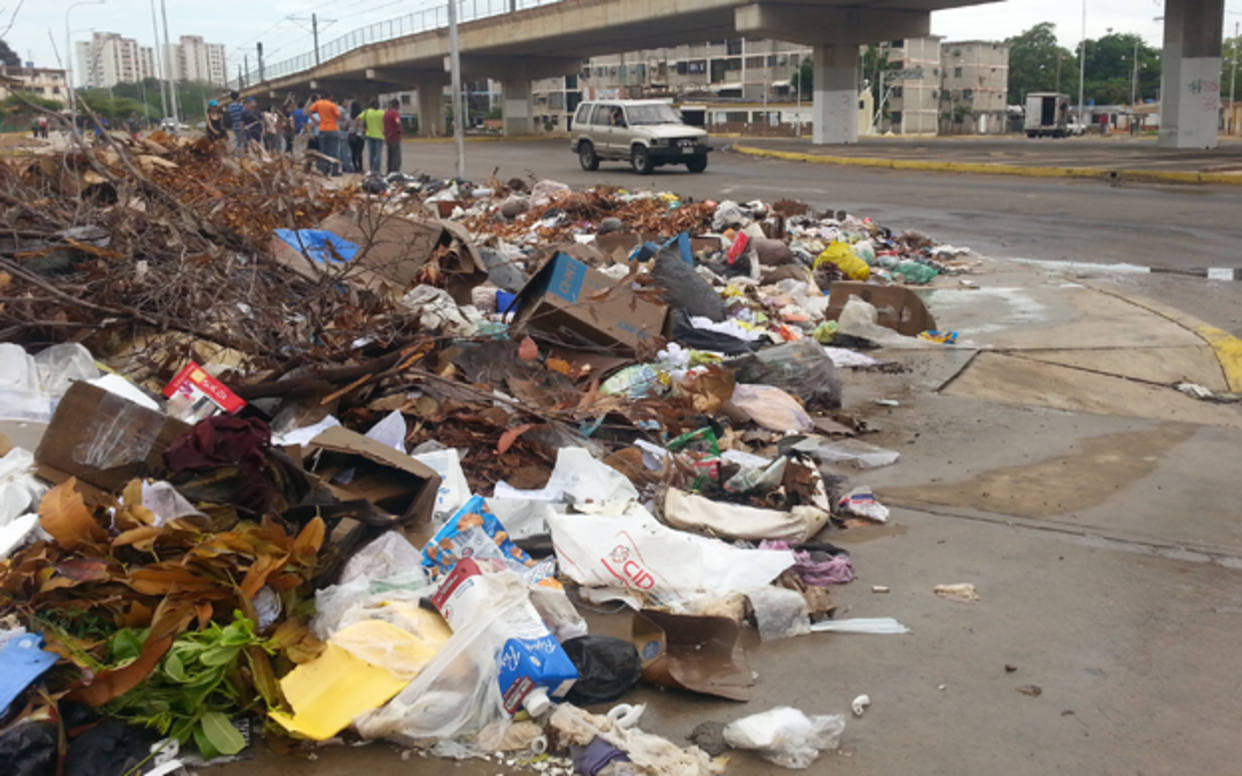
\includegraphics[width=300px]{117.jpg}%
\newline%
%
La basura en las calles de Maracaibo, en el estado Zulia, están llenas~debido al mal servicio que presta el aseo en la zona. Los vecinos amenazan con quemar los desperdicios si no se les ofrece una solución.%
\newline%
%
El camión del aseo lleva más de 18 días sin recorrer algunas calles de la ciudad como Sabaneta y Pomona. Los habitantes denuncian que ambos lugares permanecen~infestados de plaga como moscas e indican que la falta de salubridad puede ser perjudicial para su salud.%
\newline%
%
Richard Guanipa, presidente del Instituto Municipal de Aseo Urbano de Maracaibo (IMAU), informó que el retraso en el servicio ocurrió debido a una contingencia ocurrida en la ciudad, sin embargo, dijo al~Diario La Verdad~que se retomará pronto.%
\newline%
%
De igual forma, Guanipa aclaró que hay aproximadamente 300 empleados trabajando para solucionar el problema de desperdicios del lugar.%
\newline%
%
Lea más en~Diario la~Verdad.%
\newline%
%
\end{document}